\documentclass[12pt]{article}

\usepackage[margin=1in]{geometry}
\usepackage{amsmath,amssymb}
\usepackage{graphicx}
\usepackage{booktabs}
\usepackage[hyphens]{url}
\usepackage[hidelinks]{hyperref}
\usepackage{natbib}
\usepackage[table]{xcolor}
\usepackage{array}
\usepackage{bm}
\emergencystretch=1em
\setlength{\abovecaptionskip}{14pt}
\setlength{\belowcaptionskip}{12pt}

\bibliographystyle{plainnat}

\title{\bfseries Does Deep-Learning Asset Pricing Transfer to Frontier Markets?\\
A Deep Stochastic Discount Factor for Iran, T\"urkiye, and Pakistan}
\author{DLAP-TSE Research Project}
\date{\today}

\begin{document}
\maketitle

% ---------------------------------------------------------------------
\begin{abstract}
\noindent How much of modern machine-learning asset pricing survives a transfer to thin, illiquid, frontier markets? The deep-learning stochastic discount factor (SDF) of \citet{cpz2024} was estimated on a US cross-section of tens of thousands of stocks; its economic value rests on assumptions---a large, liquid cross-section, smooth price discovery, and a stable relation between characteristics and returns---that frontier markets violate by construction. We test those assumptions where they bind, on three frontier or near-frontier exchanges spanning three macro-financial regimes: the Tehran Stock Exchange (TSE; sanctions, retail-dominated trading, $\pm5\%$ daily price band), Borsa Istanbul (BIST; $\pm10\%$ band, chronic inflation), and the Pakistan Stock Exchange (PSX; shallow book, MSCI frontier classification, retail limit-ordered trading). We replicate the \textsc{cpz} construction faithfully---a common SDF $M_{t+1}=1-\frac{1}{N_t}\sum_i\omega_t(i)R^e_{t+1,i}$ with network-learned weights over characteristics and macro states, estimated by minimizing squared pricing errors---under one identical protocol in all three markets: a 60/12 rolling-window evaluation with lagged characteristics, benchmarks rebuilt from the same winsorized panels as the deep model, all characteristics lagged one month, and linear-SDF, LASSO, PCA, FF5, q-factor and market benchmarks (12 test windows in Iran, 6 in T\"urkiye and 5 in Pakistan, forced by factor availability). The transfer is sharply split. The deep SDF's \emph{pricing content} transfers: in every market its strongest specifications post the lowest or near-lowest pricing errors of any model (RMS $\alpha$ as low as @@IR:ALPHA_LOW@@\%, @@TR:ALPHA_LOW@@\% and @@PK:ALPHA_LOW@@\% monthly in Iran, T\"urkiye and Pakistan, versus @@IR:BENCH_ALPHA@@\%, @@TR:BENCH_ALPHA@@\% and @@PK:BENCH_ALPHA@@\% for the best benchmark) and its explained return variation (EV) is the highest of any characteristic-based model in all three markets. Its \emph{portfolio representation} does not: the as-trained SDF portfolio is fragile everywhere (seed spreads of @@IR:E2_RANGE@@, @@TR:E2_RANGE@@ and @@PK:E2_RANGE@@ in annualized Sharpe for the baseline specification alone), and the liquidity filter that stabilized the portfolio in our earlier single-market evidence does not transfer. What does transfer, in all three markets and all training seeds, is a \emph{sign-ambiguity mechanism}: the squared-pricing-error objective on a few hundred stocks is approximately symmetric with respect to portfolio orientation (we verify this directly by evaluating the converged objective at both orientations), and under the standard sign convention (the SDF prices the risk-free asset) the deep SDF portfolio attains Sharpes of @@SIGN_RANGE@@ in every market---stable across training seeds and competitive with the strongest factor benchmarks in each (above them in Iran and Pakistan, essentially tied with the Turkish q-factor); we report this as a diagnostic upper bound, not an implementable result. An \emph{ex-ante} sign-pinning penalty estimated from training data alone then separates weak optimization identification from genuine train-to-test instability: it improves orientation in Iran, is neutral in T\"urkiye, and fails in Pakistan---so small-market portfolio instability ranges from weak sign identification (Iran) through already-persistent orientation (T\"urkiye) to genuine train-to-test portfolio instability (Pakistan). The binding frontier-market constraint is therefore not liquidity but estimator identification: portfolio-level conclusions from small cross-sections require sign pinning or equivalent regularization before they can be read economically.
\end{abstract}

\vspace{1em}
\noindent\textbf{Keywords:} deep learning; stochastic discount factor; asset pricing; frontier markets; Tehran Stock Exchange; Borsa Istanbul; Pakistan Stock Exchange; machine learning

% ---------------------------------------------------------------------
\section{Introduction}\label{sec:intro}

A central goal of asset pricing is to explain the cross-section of expected returns with a small set of priced risks. Since \citet{hj1991}, any asset-pricing model can be viewed as a restriction on the stochastic discount factor (SDF), and \citet{cochrane2011} argued forcefully that the SDF itself---rather than a particular list of factors---is the object to estimate. Machine learning made high-dimensional SDF estimation practical: \citet{gkx2020} showed that neural networks dominate linear methods at predicting returns from firm characteristics, and \citet{cpz2024} showed that a network can estimate the SDF directly from the no-arbitrage condition, pricing individual stocks rather than pre-sorted portfolios. Every paper in this young literature, however, estimates on US (or, rarely, Chinese) data---cross-sections of thousands of liquid stocks with decades of clean price discovery. The economic content of the deep SDF rests on assumptions that such data satisfy and that most of the world's markets do not: a cross-section large enough for network weights to be identified, returns informative enough for pricing errors to be estimated, and a tradable universe liquid enough for the estimated SDF portfolio to be implementable. Whether deep-learning asset pricing \emph{transfers}---and which of its components survive when these assumptions fail---is the open scientific question this paper addresses.

We test external validity on three frontier or near-frontier exchanges chosen to span, rather than repeat, a single institutional environment: the \textbf{Tehran Stock Exchange} (TSE), the largest MENA market by listings, with sanctions-driven regime breaks, a $\pm5\%$ daily price band and retail-dominated trading; \textbf{Borsa Istanbul} (BIST), a large emerging market with a $\pm10\%$ band, persistent high inflation and an active derivatives market; and the \textbf{Pakistan Stock Exchange} (PSX), an MSCI-classified frontier market with a shallow limit-order book, no liquid derivatives, and a banking-heavy, family-controlled listing universe. These are not three draws from one market type: they differ in liquidity provision, price-limit regimes, inflation environments and factor availability, so agreement among them is evidence about the method, not about one market's idiosyncrasies. A transfer claim that survived in only one of them would be a claim about that market; a claim that survives all three is a claim about the estimator.

We replicate the \textsc{cpz} model faithfully---a \emph{common} SDF $M_{t+1}=1-\frac{1}{N_t}\sum_i \omega_t(i) R^e_{t+1,i}$ whose weights $\omega_t(i)$ are network outputs over characteristics and macro states, estimated by minimizing squared pricing errors of individual stocks---under one identical protocol in all three markets. @@ROADMAP@@ Our contributions are fivefold. \textbf{First}, we provide the first deep-learning SDF estimates for any frontier market, implemented faithfully to the \textsc{cpz} construction and---unlike single-market studies---with a pipeline in which every script, window structure, loss, alignment rule and benchmark construction is byte-identical across the three markets. \textbf{Second}, we show that the deep SDF's \emph{pricing content} transfers everywhere: in each market the deep specifications post the lowest or near-lowest RMS pricing errors of any model (Iran from @@IR:ALPHA_LOW@@\% monthly versus @@IR:BENCH_ALPHA@@\% for the best of FF5, q-factor, PCA(5), LASSO and the market; T\"urkiye from @@TR:ALPHA_LOW@@\% versus @@TR:BENCH_ALPHA@@\%; Pakistan from @@PK:ALPHA_LOW@@\% versus @@PK:BENCH_ALPHA@@\%) and the highest explained return variation (EV) of any characteristic-based model. \textbf{Third}, we show that its \emph{portfolio representation} does not transfer: the as-trained SDF portfolio is fragile in all three markets, with the baseline eleven-signal specification spanning @@IR:E2_RANGE@@ (Iran), @@TR:E2_RANGE@@ (T\"urkiye) and @@PK:E2_RANGE@@ (Pakistan) in annualized Sharpe across training seeds. \textbf{Fourth}, we show that the liquidity-filter stabilization documented in our earlier single-market evidence does not transfer: on the current bank-free Iranian panel the filter's pooled-Sharpe advantage is not statistically distinguishable from zero (bootstrap interval @@IR:BOOT_E8_LASSO@@ versus LASSO), and in neither T\"urkiye nor Pakistan does it improve the portfolio. \textbf{Fifth}, we identify what does transfer robustly: a \emph{sign-ambiguity mechanism}. The squared-pricing-error objective on a few hundred stocks leaves the sign of the SDF weights effectively unpinned; under the standard sign convention the deep SDF portfolio attains Sharpes of @@SIGN_RANGE@@ in every market---stable across training seeds and competitive with the strongest factor benchmarks in each (above them in Iran and Pakistan, essentially tied with the Turkish q-factor)---so the binding frontier-market constraint is estimator identification, not liquidity. An \emph{ex-ante} sign pin estimated from training data alone then validates the mechanism where it applies: it repairs the Iranian portfolio without any test-window information, leaves the already-stable Turkish portfolio unchanged, and fails in Pakistan---direct evidence of train-to-test sign instability in that market (Section~\ref{sec:methodb}).

Four questions organize the empirical work. \textbf{(RQ1)} Does the deep SDF's \emph{pricing content} transfer to thin frontier cross-sections: does it beat linear factor benchmarks and a linear-in-characteristics SDF out of sample on pricing errors and explained variation? \textbf{(RQ2)} Does its \emph{portfolio representation} transfer: is the estimated SDF portfolio stable across training seeds and competitive with factor portfolios, and does the liquidity filter that stabilized a single earlier panel generalize? \textbf{(RQ3)} Do the two signature elements of the \textsc{cpz} machinery---macro-state conditioning and the adversarial critic---carry over to markets of a few hundred stocks? \textbf{(RQ4)} What explains the portfolio-level failures, and what does the pattern across three markets imply for machine-learning asset pricing in frontier markets?

The paper proceeds as follows. Section~\ref{sec:lit} reviews the related literature and states what is known, what remains unknown, and why frontier markets matter. Section~\ref{sec:data} describes the three data panels, their construction and their availability constraints. Section~\ref{sec:method} lays out the model and the evaluation protocol. Section~\ref{sec:results} presents benchmark and SDF results in each market and pooled across markets. Section~\ref{sec:robust} reports robustness, seed sensitivity and mechanism evidence. Section~\ref{sec:concl} concludes with the broader implications for machine-learning asset pricing in markets where the tradable tail is thin.

% ---------------------------------------------------------------------
\section{Literature review}\label{sec:lit}

\subsection{From factor models to the stochastic discount factor}

A central theme of modern asset pricing is that all models of expected returns can be viewed as restrictions on the SDF \citep{hj1991,cochrane2011}. Two econometric innovations made high-dimensional SDF estimation practical. \citet{lettaupelger2020} introduced risk-premium PCA, which augments the standard PCA objective with a pricing-error penalty, and its rolling-window evaluation protocol---training/validation/test splits with out-of-sample Sharpe and root-mean-squared pricing errors---is the template for the evaluation below. \citet{kps2019} show that instrumented PCA, which lets factor loadings depend on characteristics, attains an out-of-sample tangency Sharpe of 3.89 versus 1.29--1.53 for characteristic-sorted factors on US data.

\subsection{Machine learning in the cross-section}

The modern machine-learning cross-section begins with \citet{gkx2020}, who compare penalized linear, tree, and neural models for predicting US returns from firm characteristics: neural networks and gradient-boosted trees dominate linear methods, and value-weighted decile-spread portfolios earn Sharpe ratios of 1.35--2.45 out of sample. \citet{kps2019} show that instrumented PCA, which lets factor loadings depend on characteristics, attains an out-of-sample tangency Sharpe of 3.89 versus 1.29--1.53 for characteristic-sorted factors on US data.

\subsection{Deep-learning stochastic discount factors}

\citet{cpz2024}---the paper we replicate---estimate the SDF with neural networks. Their model takes the form
\begin{equation}
M_{t+1} \;=\; 1 - \sum_{i=1}^{N_t} \omega_t(i)\, R^e_{t+1,i},
\label{eq:sdf}
\end{equation}
where $R^e_{t+1,i}$ is the excess return of stock $i$, and the SDF weights $\omega_t(i) = g(z_t, x_{i,t})/N_t$ are produced by a network $g$ that takes the firm's characteristics $x_{i,t}$ together with a low-dimensional macro state $z_t$ extracted from a panel of lagged macroeconomic variables. Estimation minimizes squared pricing errors $\mathbb{E}[M_{t+1}R^e_{t+1,i}]$ over all stocks rather than prediction error, and an adversarial critic network searches for the portfolio the SDF prices worst, forcing the SDF to improve where it fails. On US data the resulting SDF attains a test-period Sharpe ratio of 0.75 and an out-of-sample cross-sectional $R^2$ of 0.23.

A growing family of papers extends this approach: autoencoder models with no-arbitrage restrictions \citep{gkx2021}; tree-based sparse cross-sections \citep{bpz2025}; deep characteristic-sorted factor models \citep{fhpx2024}; variational autoencoders \citep{cwh2026}; news embeddings from pretrained language models \citep{wcw2025}; deep partial least squares \citep{dixon2022}; and deep-learning statistical arbitrage \citep{gpz2025}. On the theory side, \citet{kmz2024} prove that under misspecification the deep SDF's implicit regularization---not the network's expressiveness---determines pricing performance, a warning that transfers with extra force to small cross-sections.

\subsection{Factor models and anomalies on the three exchanges}

Each of our markets has a parametric factor-model literature; none has a machine-learning SDF. For \textbf{Iran}, \citet{talakesh2023}---explicitly the first SDF test in the country---estimate CAPM and FF3 in both beta and SDF form by GMM on 25 size--book-to-market portfolios (FF3 on 20) over 2000--2019; the FF3 SDF is the only specification not rejected ($J=20.51$, $p=0.11$). \citet{taleblou2022} estimate a behavioral SDF in which investor sentiment enters the kernel; \citet{taleblou2024} formalize sentiment (measured by turnover) as a priced risk factor; \citet{davallou2015} reject CAPM, FF3, and Carhart on TSE test assets. For \textbf{T\"urkiye}, tests of the Fama--French three-factor model on Borsa Istanbul find that it explains time-series portfolio returns well but leaves the cross-section of individual stock returns largely unexplained \citep{cobanoglu2025}, with related evidence on share issuance \citep{atilgan2016} and on the three-factor model's early-sample validity \citep{guzeldere2012,aras2018}. For \textbf{Pakistan}, style-portfolio studies document persistent size and value premia that neither FF3/FF5 nor business-cycle variables explain \citep{kashif2023}, and three-factor tests on the KSE-100 reach similar conclusions \citep{abbas2015}. Across all three markets the parametric literature stops at linear factor models and sorted portfolios.

\subsection{Deep learning on the three exchanges: prediction without pricing}

Deep learning is mature on all three markets' \emph{data}---but only as a prediction technology. On Iranian data, from the earliest comparisons of networks with factor models as forecasters \citep{chavoshi2003,namazi2007,azar2010,esfahanipour2011} through the modern LSTM/CNN/GRU and reinforcement-learning wave \citep{nabipour2020,hadizadeh2023,tehrani2025,osoolian2025,raefi2018}, the most telling entry is \citet{heidari2022}: a seventeen-model horse race on 150 TSE stocks whose best LSTM reaches 75.1\% directional accuracy---a strong forecasting result that, like the rest of this literature, stops short of pricing. The Turkish and Pakistani literatures are similarly prediction-centric, and none of these studies estimates an SDF, evaluates a no-arbitrage pricing kernel, or asks what the learned patterns imply for the cross-section of expected returns.

\subsection{What is known, what remains unknown, and why frontier markets matter}

Three facts anchor this literature. \emph{First}, on large, liquid markets---primarily the US---machine learning dominates linear methods for return prediction \citep{gkx2020} and for SDF estimation \citep{cpz2024}, and the deep SDF prices individual stocks rather than pre-sorted portfolios. \emph{Second}, the deep SDF's success is associated with two design features---macro-state conditioning and an adversarial critic---whose contribution is documented on US data but not elsewhere. \emph{Third}, the transfer evidence is confined to large markets: no deep SDF has been estimated on any frontier or MENA exchange, and the extensive Iranian machine-learning literature is entirely predictive. What remains unknown is precisely what a transfer study can establish: whether the deep SDF's \emph{pricing content} survives a two-order-of-magnitude reduction in cross-section size; whether its \emph{portfolio representation} survives when the tradable universe is thin and returns are truncated by price limits; and whether the design elements that matter in the US carry economic value elsewhere. These questions matter beyond any single market because the deep SDF's practical constituency is not the US---where liquid factor portfolios already exist---but precisely the small, illiquid markets in which machine-learning pricing could substitute for absent institutional research. Existing evidence cannot answer them: every published estimate comes from a market large enough to make the failure modes we study invisible. Three exchanges with different institutional frictions, studied under one identical pipeline, are the sharpest available laboratory for that test.

% ---------------------------------------------------------------------
\section{Data}\label{sec:data}

\subsection{Three panels, one pipeline}\label{sec:coverage}

The three panels differ in length, breadth and data availability; the pipeline that consumes them is identical. Table~\ref{tab:coverage} summarizes. The \textbf{Iran} panel is built from official TSETMC monthly data, adjusted for dividends and capital increases (raw adjustment spikes reach $+1{,}692\%$ in a single month, which winsorization and the missing-return treatment remove). The \textbf{T\"urkiye} panel is built from BIST price files via the EVDS API with financials from KAP; the \textbf{Pakistan} panel from PSX end-of-day data with financial statements extracted from annual reports by a vision-language-model pipeline with a three-layer quality-assurance audit (parser--VLM conflict review, external cross-checks against the exchange's own dividend records, and per-symbol manifests); @@PK_COVERAGE@@.

\begin{table}[htbp]
\centering
\caption{Three-market data coverage. ``Common period'' is the span over which the return panel and both factor sets (FF5 and q-factor) are simultaneously available; the out-of-sample (OOS) test windows are the 12-month rolling windows that fit after the 60-month training lookback. @@WIN_NOTE@@}
\label{tab:coverage}
\small
\setlength{\tabcolsep}{4pt}
\begin{tabular}{lccc}
\toprule
 & Iran (TSE) & T\"urkiye (BIST) & Pakistan (PSX) \\
\midrule
Panel span & @@IR:PANEL_SPAN@@ & @@TR:PANEL_SPAN@@ & @@PK:PANEL_SPAN@@ \\
Stocks (full panel) & @@IR:N_STOCKS@@ & @@TR:N_STOCKS@@ & @@PK:N_STOCKS@@ \\
Stock-months & @@IR:SM@@ & @@TR:SM@@ & @@PK:SM@@ \\
Characteristics & 20 & 20 & 19 \\
Common period & @@IR:COMMON@@ & @@TR:COMMON@@ & @@PK:COMMON@@ \\
Common months & @@IR:T_COMMON@@ & @@TR:T_COMMON@@ & @@PK:T_COMMON@@ \\
FF5/q factors from & 2008-07 & 2015-07 & 2014-10 \\
OOS test windows & @@IR:NWIN@@ (2013-07--2025-06) & @@TR:NWIN@@ (2020-07--2026-06) & @@PK:NWIN@@ (2019-10--2025-09) \\
OOS test months & @@IR:OOSM@@ & @@TR:OOSM@@ & @@PK:OOSM@@ \\
Macro series & 6 & 6 & 6 \\
HJ bound (monthly) & @@IR:HJ@@ & @@TR:HJ@@ & @@PK:HJ@@ \\
\bottomrule
\end{tabular}
\end{table}

\subsection{Characteristics and their availability}\label{sec:chars}

We use twenty firm characteristics, cross-sectionally z-scored each month and winsorized at the 1\%/99\% level, identical in name and construction across the three markets wherever the underlying data permit. Eleven are the Stambaugh--Yuan (SY) mispricing signals \citep{sy2017}: net stock issuance, composite equity issuance, accruals, net operating assets, asset growth, investment-to-assets, investment growth, distress, O-score, momentum, and gross profitability. Nine further characteristics follow the machine-learning cross-section conventions \citep{gkx2020,cpz2024}: size, book-to-market (BE/ME), short-term continuation, ROE, investment (I/A), cash-based operating profitability, dividend yield, turnover, and volatility. Exact definitions are in Appendix~\ref{app:chars}. All accounting characteristics are aligned to returns through the formation-year convention (month $m\ge7$ of year $y$ uses formation year $y$; month $m<7$ uses $y-1$), eliminating look-ahead bias.

Two availability constraints bind, and we document them explicitly. \emph{First}, \textbf{Pakistan's long-term-investment data do not support the investment-growth (IG) characteristic}: the annual-report extraction yields usable long-term-investment values for only @@PK:LT_INV_COV@@ of firm-years, so PSX panels carry 19 characteristics (18 in the z-scored estimation set after dropping the near-empty dividend-yield series); the LASSO design matrix there further drops characteristics with below-30\% coverage, leaving 18 usable characteristics for LASSO and a 10-signal SY subset for the linear SDF. \emph{Second}, \textbf{the factor benchmarks start late in T\"urkiye and Pakistan}: FF5 and q-factor portfolios require formation-year accounting data, which begin in 2015-07 on BIST and 2014-10 on PSX (versus 2008-07 on TSE). Because the protocol trains on 60 months and tests on 12, this compresses the OOS evaluation to @@TR:NWIN@@ windows in T\"urkiye (2020-07--2026-06) and @@PK:NWIN@@ in Pakistan (2019-10--2025-09) versus @@IR:NWIN@@ in Iran (2013-07--2025-06). We treat these as properties of the data-generating environment---part of what ``frontier market'' means---and report every model on the windows its inputs permit; @@PK_SHORT_NOTE@@

\subsection{Return treatment and price limits}

TSE returns are computed from officially adjusted prices; daily moves are bounded by the $\pm5\%$ band (an institutional feature we do not correct), a handful of post-adjustment extremes (returns below $-50\%$) are treated as missing, and monthly returns are winsorized cross-sectionally at the 1/99 percentiles. BIST raw series contain split-related jumps of up to $+702\%$, which the same 1/99 winsorization absorbs. PSX panels apply identical winsorization and the same $-50\%$ missing-return rule. All three panels therefore enter the estimator in the same units, winsorized by the same rule, with the same lag alignment and the same train/validate/test geometry (Section~\ref{sec:method}).

\subsection{Macro panels}

Each market's state-extraction network consumes six monthly macro series chosen for that market's institutional environment. \textbf{Iran}: the CBI policy rate, CPI (2010=100), the official USD/IRR rate, Brent crude, the Emami gold coin price, and the market (free-market) USD/IRR rate. \textbf{T\"urkiye}: the CBRT policy rate, CPI, USD/TRY, the 3-month T-bill rate, Brent crude, and M2. \textbf{Pakistan}: the SBP policy rate (IMF IFS through 2021-12, SBP monetary-policy statements thereafter, with a documented $\approx$1pp definitional seam), CPI, USD/PKR, the 6-month T-bill, Brent crude, and the KSE-100 index level. All series are monthly, normalized with training-window moments, and missing early observations are forward-filled.

% ---------------------------------------------------------------------
\section{Methodology}\label{sec:method}

\subsection{The deep SDF}

We follow \citet{cpz2024}. The SDF is a \emph{common} pricing kernel over all stocks,
\begin{equation}
M_{t+1} \;=\; 1 - \frac{1}{N_t}\sum_{i=1}^{N_t} \omega_t(i)\, R^e_{t+1,i},
\label{eq:sdf2}
\end{equation}
where $N_t$ is the number of stocks with valid data in month $t$ and the SDF weight of stock $i$,
\begin{equation}
\omega_t(i) \;=\; g\bigl(z_t,\, x_{i,t}\bigr),
\label{eq:omega}
\end{equation}
is the output of a feedforward network $g$ (the \emph{weight network}) that takes the stock's characteristics $x_{i,t}\in\mathbb{R}^F$ together with a macro state $z_t\in\mathbb{R}^4$ extracted by a one-layer LSTM over the six macro series (the \emph{state network}), trained jointly. The weight network has two hidden layers of 64 units with ReLU activations and dropout with keep probability 0.95, matching the official \textsc{cpz} configuration. Note that the SDF in \eqref{eq:sdf2} is a single scalar per month---the same kernel prices every stock---and that the network's nonlinearity acts on the characteristics themselves (through $x_{i,t}$), not only on the state. The no-arbitrage restriction is imposed on \emph{excess} returns, $\mathbb{E}_t[M_{t+1}R^e_{i,t+1}]=0$ (equivalent to $\mathbb{E}_t[M_{t+1}R_{i,t+1}]=1$ when the risk-free asset is priced); given the normalization $M_t = 1 - (\text{portfolio component})$, this condition pins down the portfolio component of $M$ up to orientation and scale, while the level (the price of the risk-free asset) is fixed by the constant 1. Concretely: the \emph{pricing-kernel moments} are identified, the \emph{portfolio orientation} is not (Section~\ref{sec:signconv}), and the scale of the portfolio component is set by the unit-gross-leverage convention on the reported SDF portfolio. For each stock, the pricing error is
\begin{equation}
\alpha_i \;=\; \frac{1}{T_i}\sum_{t\in\mathcal{T}_i} M_t\, R^e_{i,t},
\label{eq:alpha}
\end{equation}
where $R^e$ is the excess return and $\mathcal{T}_i$ the set of months in which stock $i$ is observed (at least six required), and the loss is the weighted mean squared pricing error $\frac{1}{N}\sum_i (c_i/\max_j c_j)\, \alpha_i^2$ with $c_i=|\mathcal{T}_i|$, the observation-count weighting of the official \textsc{cpz} implementation. Training uses Adam with learning rate $10^{-3}$, a maximum of 400 epochs, and early stopping on the validation-window pricing error (patience 25).

For the adversarial-critic specification (E5), a \emph{moment network} $h(z_t,x_{i,t})\in\mathbb{R}^8$ with $\tanh$ output---the official \textsc{cpz} critic---searches for eight characteristic-conditional portfolios on which the SDF prices worst: it maximizes $\sum_{k,i} [\frac{1}{T_i}\sum_t h_k(z_t,x_{i,t}) M_t R^e_{i,t}]^2$, while the SDF minimizes the same object (alternating Adam updates, loss weight 1.0).

\subsection{Specifications}

Eight deep specifications, identical across markets, cross the three design elements: character set (E2/E4B/E5A/E8 use the 11 SY mispricing signals; E3/E4A/E5B/E8B use all 20 characteristics), state network (LSTM macro states or a learned constant), critic (on/off), and liquidity filter (E8/E8B exclude the bottom 5\% of stocks by train-window turnover). Three training seeds (42, 43, 44) are run for every specification in every market.

\subsection{Evaluation protocol}

All models are evaluated under the rolling-window protocol of the machine-learning asset-pricing canon \citep{lettaupelger2020,gkx2020}: for each non-overlapping twelve-month test window (@@IR:NWIN@@ windows in Iran, @@TR:NWIN@@ in T\"urkiye, @@PK:NWIN@@ in Pakistan), deep SDFs are estimated on the preceding forty-eight months with the preceding twelve months held out for early stopping (a sixty-month lookback in total), and linear benchmarks are estimated on the full sixty months. Three out-of-sample metrics are computed, pooled across test windows:
\begin{itemize}
\item \textbf{SDF-portfolio Sharpe ratio} (annualized): the Sharpe ratio of the SDF-implied portfolio return
\begin{equation}
r_{p,t} \;=\; \frac{\sum_i \omega_t(i)\, R^e_{i,t}}{\sum_i |\omega_t(i)|},
\label{eq:rp}
\end{equation}
i.e.\ the zero-cost portfolio with weights proportional to the SDF weights, at unit gross leverage. The same normalization is applied to the factor benchmarks (maximum-Sharpe weights $w=\Sigma^{-1}\mu$ with covariance shrunk toward the diagonal, $\delta=0.2$), whose raw weights carry arbitrary leverage (mean gross exposure @@IR:FF5_LEV@@ in Iran and @@TR:FF5_LEV@@ in T\"urkiye for FF5); portfolio-level objects other than the Sharpe ratio are therefore compared at unit gross leverage.
\item \textbf{Explained return variation (EV)}: for each test window, regress each stock's returns on the model's SDF portfolio return and compute $1 - SS_{res}/SS_{tot}$ pooled over stocks and windows. The regression is fit within the test window, so EV is a \emph{descriptive test-period fit measure}, not a predictive out-of-sample $R^2$; it uses the same construction for every model, and we report it as such throughout.
\item \textbf{Pricing errors}: $\alpha_i = \frac{1}{T_i}\sum_t M_t R^e_{i,t}$ on test months, with the common SDF of \eqref{eq:sdf2}; we report the pooled RMS and maximum absolute value, and the Hansen--Jagannathan bound of the test assets (@@IR:HJ@@ monthly in Iran, @@TR:HJ@@ in T\"urkiye, @@PK:HJ@@ in Pakistan) as the theoretical maximum Sharpe ratio.
\end{itemize}
Benchmarks are FF5 \citep{ff2015}, the q-factor model \citep{hxz2015} (constructed from $2\times3$ value-weighted sorts on size$\times$I/A and size$\times$ROE with all-stock breakpoints), five principal components of returns, LASSO on the characteristic panel ($\lambda$ chosen by three-fold cross-validation within each training window), the market (CAPM reference), and a \emph{linear SDF} benchmark---the common SDF \eqref{eq:sdf2}--\eqref{eq:alpha} with $\omega_t(i)=\theta' x_{i,t}$, $\theta\in\mathbb{R}^F$ estimated in closed form by the same weighted squared-pricing-error loss on the training window. The linear SDF is the parametric restriction of the deep model and is the natural benchmark against which the network's nonlinearity is judged. For LASSO we implement cyclic coordinate descent (Gauss--Seidel) with warm starts.

\paragraph{Implementation.} All deep-SDF models are estimated in PyTorch on CPU (a two-core machine), with \texttt{torch.manual\_seed(42)} fixing the global seed and the same seed used in the LASSO cross-validation. Each window uses 48 training months, the preceding 12 months for validation, and the following 12 months as the test window. The estimation, evaluation, and artifact-generation scripts are country-parameterized by a single environment variable, and every deep run is repeated at seeds 42, 43 and 44. The complete replication package (scripts and results) is publicly available at \url{https://github.com/amirziveh/dlap-tse}.

% ---------------------------------------------------------------------
\section{Results}\label{sec:results}

\subsection{Benchmarks: linear factor models are weak or unstable in all three markets}\label{sec:bench}

Table~\ref{tab:bench} reports out-of-sample performance of the benchmark models, all built from the same winsorized return panels as the deep SDF, and Table~\ref{tab:deep} reports the deep specifications. Four facts stand out. \emph{First}, linear factor models are weak or unstable everywhere. In Iran the best benchmark is the q-factor at Sharpe @@IR:Q@@, with FF5 at @@IR:FF5@@ and the market at @@IR:MKT@@---far below the Hansen--Jagannathan bound of @@IR:HJ_ANN@@ annualized. In T\"urkiye the q-factor earns @@TR:Q@@ and the market @@TR:MKT@@, but the \emph{same} market portfolio loses money in the fifth test window (per-window Sharpe $-2.89$); in Pakistan the market earns @@PK:MKT@@ and FF5 \emph{negative} @@PK:FF5@@. \emph{Second}, the linear characteristic SDF is now the strongest benchmark class in Iran (Sharpe @@IR:LIN11@@ with 11 signals and @@IR:LIN20@@ with 20)---@@LIN_STRENGTH_NOTE@@---and reaches @@PK:LIN20@@ in Pakistan with 19 characteristics, while it remains weak in T\"urkiye (@@TR:LIN20@@). \emph{Third}, no linear model in any market delivers both a competitive portfolio and competitive pricing errors: the linear SDF's RMS $\alpha$ (@@IR:LIN20_ALPHA@@\% in Iran, @@TR:LIN20_ALPHA@@\% in T\"urkiye, @@PK:LIN20_ALPHA@@\% in Pakistan) is the worst or near-worst in its market wherever its Sharpe is strong, a trade-off the deep model escapes. \emph{Fourth}, the strict out-of-sample cross-sectional $R^2$ (training-window betas and premia applied to test means) is negative for every benchmark in every market ($-0.4$ to $-2.8$), so no linear model explains the cross-section out of sample anywhere; EV, a different construction (a descriptive test-period regression fit, Section~\ref{sec:method}), is positive throughout and is the highest for the deep SDF among characteristic-based models in all three markets.

\begin{table}[htbp]
\centering
\footnotesize
\setlength{\tabcolsep}{4pt}
\caption{Out-of-sample benchmark performance by market (Sharpe and EV pooled over each market's OOS windows; RMS $\alpha$ in \% monthly; all factor portfolios built from the same winsorized panels as the deep SDF; the linear SDF is the common kernel \eqref{eq:sdf2} with $\omega=\theta'x$). HJ = Hansen--Jagannathan bound of the test assets, monthly.}
\label{tab:bench}
\scriptsize
\setlength{\tabcolsep}{3pt}
\begin{tabular}{l cccc cccc cccc}
\toprule
 & \multicolumn{4}{c}{Iran} & \multicolumn{4}{c}{T\"urkiye} & \multicolumn{4}{c}{Pakistan} \\
\cmidrule(lr){2-5}\cmidrule(lr){6-9}\cmidrule(lr){10-13}
Model & Sharpe & EV & $\alpha$ & max$|\alpha|$ & Sharpe & EV & $\alpha$ & max$|\alpha|$ & Sharpe & EV & $\alpha$ & max$|\alpha|$ \\
\midrule
Market & @@IR:R:Market@@ & @@IR:E:Market@@ & @@IR:A:Market@@ & @@IR:M:Market@@ & @@TR:R:Market@@ & @@TR:E:Market@@ & @@TR:A:Market@@ & @@TR:M:Market@@ & @@PK:R:Market@@ & @@PK:E:Market@@ & @@PK:A:Market@@ & @@PK:M:Market@@ \\
FF5 & @@IR:R:FF5@@ & @@IR:E:FF5@@ & @@IR:A:FF5@@ & @@IR:M:FF5@@ & @@TR:R:FF5@@ & @@TR:E:FF5@@ & @@TR:A:FF5@@ & @@TR:M:FF5@@ & @@PK:R:FF5@@ & @@PK:E:FF5@@ & @@PK:A:FF5@@ & @@PK:M:FF5@@ \\
q-factor & @@IR:R:q-factor@@ & @@IR:E:q-factor@@ & @@IR:A:q-factor@@ & @@IR:M:q-factor@@ & @@TR:R:q-factor@@ & @@TR:E:q-factor@@ & @@TR:A:q-factor@@ & @@TR:M:q-factor@@ & @@PK:R:q-factor@@ & @@PK:E:q-factor@@ & @@PK:A:q-factor@@ & @@PK:M:q-factor@@ \\
PCA(5) & @@IR:R:PCA(5)@@ & @@IR:E:PCA(5)@@ & @@IR:A:PCA(5)@@ & @@IR:M:PCA(5)@@ & @@TR:R:PCA(5)@@ & @@TR:E:PCA(5)@@ & @@TR:A:PCA(5)@@ & @@TR:M:PCA(5)@@ & @@PK:R:PCA(5)@@ & @@PK:E:PCA(5)@@ & @@PK:A:PCA(5)@@ & @@PK:M:PCA(5)@@ \\
LASSO & @@IR:R:LASSO@@ & @@IR:E:LASSO@@ & @@IR:A:LASSO@@ & @@IR:M:LASSO@@ & @@TR:R:LASSO@@ & @@TR:E:LASSO@@ & @@TR:A:LASSO@@ & @@TR:M:LASSO@@ & @@PK:R:LASSO@@ & @@PK:E:LASSO@@ & @@PK:A:LASSO@@ & @@PK:M:LASSO@@ \\
Linear SDF (SY) & @@IR:R:Linear SDF (11ch)@@ & @@IR:E:Linear SDF (11ch)@@ & @@IR:A:Linear SDF (11ch)@@ & @@IR:M:Linear SDF (11ch)@@ & @@TR:R:Linear SDF (11ch)@@ & @@TR:E:Linear SDF (11ch)@@ & @@TR:A:Linear SDF (11ch)@@ & @@TR:M:Linear SDF (11ch)@@ & @@PK:R:Linear SDF (11ch)@@ & @@PK:E:Linear SDF (11ch)@@ & @@PK:A:Linear SDF (11ch)@@ & @@PK:M:Linear SDF (11ch)@@ \\
Linear SDF (all) & @@IR:R:Linear SDF (20ch)@@ & @@IR:E:Linear SDF (20ch)@@ & @@IR:A:Linear SDF (20ch)@@ & @@IR:M:Linear SDF (20ch)@@ & @@TR:R:Linear SDF (20ch)@@ & @@TR:E:Linear SDF (20ch)@@ & @@TR:A:Linear SDF (20ch)@@ & @@TR:M:Linear SDF (20ch)@@ & @@PK:R:Linear SDF (20ch)@@ & @@PK:E:Linear SDF (20ch)@@ & @@PK:A:Linear SDF (20ch)@@ & @@PK:M:Linear SDF (20ch)@@ \\
\midrule
HJ bound (monthly) & \multicolumn{4}{c}{@@IR:HJ@@} & \multicolumn{4}{c}{@@TR:HJ@@} & \multicolumn{4}{c}{@@PK:HJ@@} \\
\bottomrule
\end{tabular}
\end{table}

\paragraph{Why no IPCA benchmark.} \citet{kps2019}'s instrumented PCA is the natural fifth benchmark: it lets factor loadings depend on characteristics and, on US data, dominates characteristic-sorted factors out of sample \citep{kps2019}. We exclude it deliberately, on three grounds. \emph{First}, our estimation panels hold 316--484 stocks and each training window supplies only 48 months, so IPCA's factor-mimicking reconstruction would be re-estimated every window on a $T\times N$ panel that is nearly square, with the number of estimated parameters approaching the number of observations; the literature's implementation guidance and simulation evidence is for panels with $N$ in the thousands, and nothing is known about the estimator's behavior at frontier-market dimensions. \emph{Second}, every benchmark here is estimated by the \emph{same} estimator class the deep model minimizes---the squared pricing-error loss with lagged characteristics---so differences are attributable to functional form rather than to an auxiliary modeling choice (the LASSO and linear-SDF benchmarks already cover the linear-in-characteristics null). \emph{Third}, IPCA requires a characteristic $\times$ instrument matrix per window; with 11--20 characteristics per market and our window structure this multiplies the number of design choices precisely where we have no data-driven way to select among them, so any IPCA result we reported would carry an unquantified researcher degree of freedom. We therefore read IPCA as a complementary US-scale design rather than a transferable benchmark, and note it as the most obvious extension for markets with deeper panels.

\subsection{The deep SDF: pricing content transfers, portfolios do not}\label{sec:deep}

Across all three markets the deep SDF's \emph{pricing} performance is the most robust object we measure. Deep specifications attain the lowest or near-lowest RMS $\alpha$ in every market---@@IR:ALPHA_LOW@@--@@IR:ALPHA_HIGH@@\% monthly in Iran (best benchmark @@IR:BENCH_ALPHA@@\%), @@TR:ALPHA_LOW@@--@@TR:ALPHA_HIGH@@\% in T\"urkiye (best benchmark @@TR:BENCH_ALPHA@@\%), and @@PK:ALPHA_LOW@@--@@PK:ALPHA_HIGH@@\% in Pakistan (best benchmark @@PK:BENCH_ALPHA@@\%)---and the highest EV among characteristic-based models everywhere (Iran @@IR:EV_LOW@@--@@IR:EV_HIGH@@; T\"urkiye @@TR:EV_LOW@@--@@TR:EV_HIGH@@; Pakistan @@PK:EV_LOW@@--@@PK:EV_HIGH@@). This is the \textsc{cpz} headline result surviving the frontier transfer: the no-arbitrage kernel remains a competitive pricing technology on cross-sections two orders of magnitude smaller than the US panel, under three different price-limit and inflation regimes.

The \emph{portfolio} story is the opposite. Table~\ref{tab:deep} shows the seed spread of every specification. In Iran, the baseline E2 spans @@IR:E2_RANGE@@ across seeds 42--44 and the liquidity-filtered E8 spans @@IR:E8_RANGE@@, overlapping E2's range entirely; the 95\% bootstrap interval for E8 versus LASSO is @@IR:BOOT_E8_LASSO@@, indistinguishable from zero. In T\"urkiye, E2 spans @@TR:E2_RANGE@@ and E8 @@TR:E8_RANGE@@, again overlapping, but E8 is significantly \emph{below} FF5 (@@TR:BOOT_E8_FF5@@; the paired bootstrap excludes LASSO on the shorter Turkish LASSO series). In Pakistan, E2 spans @@PK:E2_RANGE@@ while E8 spans @@PK:E8_RANGE@@---in this market the filter's mean effect is \emph{negative}---and neither specification significantly outperforms any strong benchmark: both are significantly \emph{below} PCA(5) (E2 @@PK:BOOT_E2_PCA@@; E8 @@PK:BOOT_E8_PCA@@), while every other pairwise interval spans zero. @@LIQ_TRANSFER_NOTE@@

\begin{table}[htbp]
\centering
\footnotesize
\setlength{\tabcolsep}{3.5pt}
\caption{Deep SDF specifications by market: pooled Sharpe at seeds 42/43/44 (E2 baseline: 11 SY signals, LSTM states; E3: 20 characteristics; E4A/E4B: constant states; E5A/E5B: adversarial critic; E8/E8B: liquidity-filtered, bottom 5\% by turnover excluded). Bold marks the market's best benchmark Sharpe for reference.}
\label{tab:deep}
\begin{tabular}{l ccc ccc ccc}
\toprule
 & \multicolumn{3}{c}{Iran} & \multicolumn{3}{c}{T\"urkiye} & \multicolumn{3}{c}{Pakistan} \\
\cmidrule(lr){2-4}\cmidrule(lr){5-7}\cmidrule(lr){8-10}
Spec & s42 & s43 & s44 & s42 & s43 & s44 & s42 & s43 & s44 \\
\midrule
@@DEEP_TABLE_ROWS@@
\midrule
\multicolumn{10}{l}{\emph{Benchmarks for reference:}} \\
q-factor & @@IR:Q@@ & & & @@TR:Q@@ & & & @@PK:Q@@ & & \\
LASSO & @@IR:LASSO@@ & & & @@TR:LASSO@@ & & & @@PK:LASSO@@ & & \\
\bottomrule
\end{tabular}
\end{table}

Table~\ref{tab:boot} reports the full pairwise moving-block bootstrap of Sharpe differences against the five benchmarks in every market (block length 6, 10{,}000 replications, seed 42, identical block indices for both legs of each pair).

\begin{table}[htbp]
\centering
\scriptsize
\setlength{\tabcolsep}{2.5pt}
\caption{Moving-block bootstrap of pooled Sharpe differences, deep SDF minus benchmark (block 6, 10{,}000 replications, seed 42; 95\% percentile intervals in brackets). ``LASSO'' pairs are absent for T\"urkiye and Pakistan because the paired series requirement cannot be met on the shorter Turkish and Pakistani LASSO evaluation windows. Intervals excluding zero would indicate a significant difference; none of the intervals that matter for the transfer conclusion excludes zero in the deep SDF's favor.}
\label{tab:boot}
@@BOOT_TABLE_ROWS@@
\end{table}

Table~\ref{tab:sign} reports the sign-convention analysis, and Figure~\ref{fig:sign} the per-window sign-normalized series. @@SIGN_PARA@@

\begin{figure}[htbp]
\centering
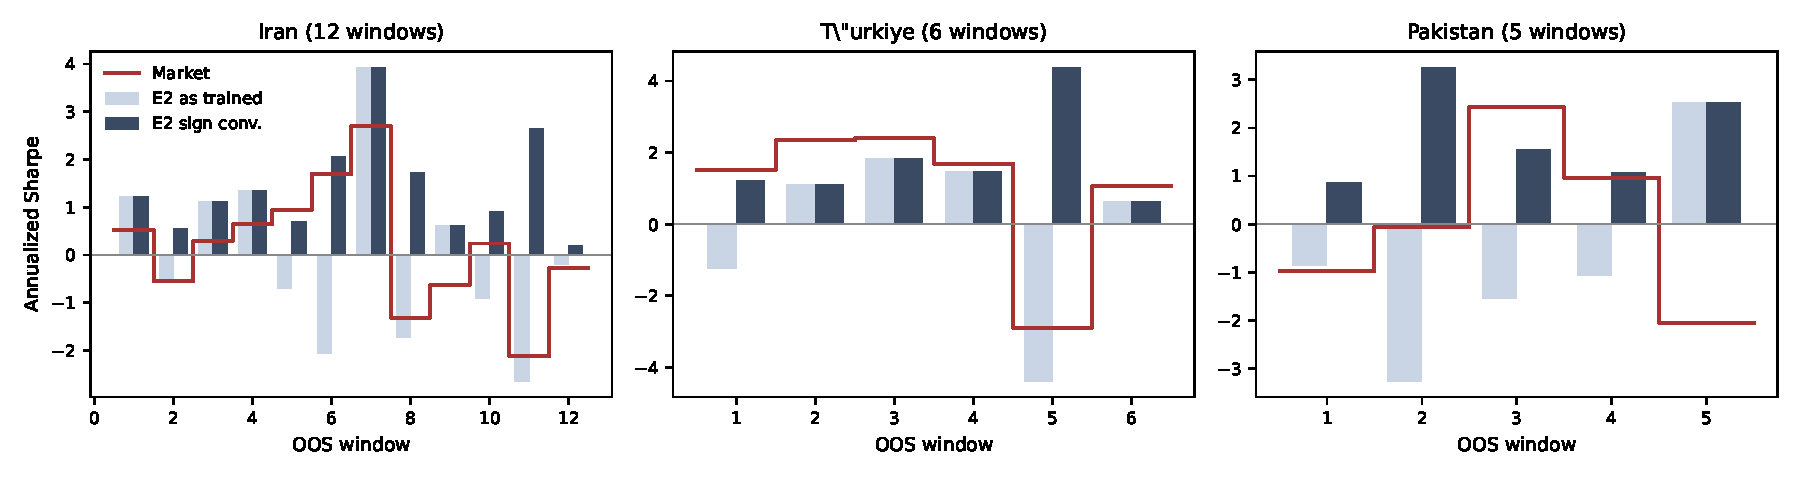
\includegraphics[width=\textwidth]{figures/fig_sign_windows.pdf}
\caption{Annualized Sharpe ratio per OOS test window of the baseline E2 deep SDF as trained (light) and under the per-window sign convention (dark), with the market benchmark (dashed) for reference. Left: Iran (@@IR:NWIN@@ windows). Center: T\"urkiye. Right: Pakistan (@@PK:NWIN@@ windows). The as-trained series are erratic, with entire windows at deeply negative Sharpe; under the sign convention the deep SDF's per-window Sharpe exceeds the market's in @@SIGN_WIN_COUNT@@ of @@TOTAL_WINDOWS@@ windows across the three markets.}
\label{fig:sign}
\end{figure}

\begin{table}[htbp]
\centering
\small
\caption{Sign-convention analysis of the SDF portfolio. ``As trained'': pooled Sharpe at the benchmark seed (42) with range across seeds 42--44. ``Sign conv.'': the same portfolio after flipping each window's weights whose mean return is negative (the SDF prices the risk-free asset, $\mathbb{E}[M]\approx 1$). ``Ex-ante pinned'': E2 retrained with the sign-pinning penalty $\lambda\,\mathrm{relu}(-\bar r^{\mathrm{train}}_p)^2$, $\lambda{=}1$ (seed 42; seed mean and sign-convention Sharpe of the pinned series in the ``Sign conv.''\ column; Section~\ref{sec:methodb}). The sign-normalized E2 is above the strongest factor benchmark in Iran and Pakistan and essentially tied with it (the q-factor) in T\"urkiye; its only superiors anywhere are @@SIGN_SUPERIORS@@.}
\label{tab:sign}
\footnotesize
\begin{tabular}{l cc cc cc}
\toprule
 & \multicolumn{2}{c}{Iran} & \multicolumn{2}{c}{T\"urkiye} & \multicolumn{2}{c}{Pakistan} \\
\cmidrule(lr){2-3}\cmidrule(lr){4-5}\cmidrule(lr){6-7}
 & As trained & Sign conv. & As trained & Sign conv. & As trained & Sign conv. \\
\midrule
E2 (11ch, LSTM) & @@IR:E2_42@@ & @@IR:SIGN_E2@@ & @@TR:E2_42@@ & @@TR:SIGN_E2@@ & @@PK:E2_42@@ & @@PK:SIGN_E2@@ \\
E8 (liq-filtered) & @@IR:E8_42@@ & @@IR:SIGN_E8@@ & @@TR:E8_42@@ & @@TR:SIGN_E8@@ & @@PK:E8_42@@ & @@PK:SIGN_E8@@ \\
E2, ex-ante pinned ($\lambda{=}1$) & @@IR:E2PIN_42@@ & @@IR:E2PIN_SN@@ & @@TR:E2PIN_42@@ & @@TR:E2PIN_SN@@ & @@PK:E2PIN_42@@ & @@PK:E2PIN_SN@@ \\
\midrule
\multicolumn{7}{l}{\emph{Benchmarks (pooled Sharpe):} q-factor @@IR:Q@@ / @@TR:Q@@ / @@PK:Q@@; LASSO @@IR:LASSO@@ / @@TR:LASSO@@ / @@PK:LASSO@@;} \\
\multicolumn{7}{l}{market @@IR:MKT@@ / @@TR:MKT@@ / @@PK:MKT@@ (Iran / T\"urkiye / Pakistan).} \\
\bottomrule
\end{tabular}
\end{table}

\begin{table}[htbp]
\centering
\small
\caption{Ex-ante sign identification (Method B, Section~\ref{sec:methodb}): the baseline E2 retrained with the training-only sign-pinning penalty, $\lambda\,\mathrm{relu}(-\bar r^{\mathrm{train}}_p)^2$. ``As trained'': unpinned E2 pooled Sharpe at each seed. ``Pinned'': with the penalty at $\lambda{=}1$. ``Sign agree.'': windows per seed in which the pinned portfolio's sign matches the ex-post per-window convention. ``SN (42)'': sign-convention Sharpe of the pinned seed-42 series; $\bar{S}$: pinned seed mean; $\bar{S}_{10}$: pinned seed mean at $\lambda{=}10$. No test-window information enters estimation.}
\label{tab:methodb}
\footnotesize
\setlength{\tabcolsep}{3pt}%
@@METHODB_TABLE_ROWS@@
\end{table}

\begin{table}[htbp]
\centering
\small
\caption{The three markets as three identification regimes. ``Pricing transfer'': pricing errors and EV relative to benchmarks (Table~\ref{tab:bench}, Table~\ref{tab:deep}). ``Raw portfolio'': as-trained seed stability (Table~\ref{tab:deep}). ``Ex-ante pin'': effect of the training-only sign-pinning penalty (Table~\ref{tab:methodb}).}
\label{tab:diagnosis}
\footnotesize
\begin{tabular}{l llll}
\toprule
Market & Pricing transfer & Raw portfolio & Ex-ante pin & Diagnosis \\
\midrule
Iran & Strong & Unstable & Improves & Weak sign identification \\
T\"urkiye & Strong & Relatively stable & Neutral & Orientation already persistent \\
Pakistan & Competitive & Unstable & Fails & Train-to-test portfolio instability \\
\bottomrule
\end{tabular}
\end{table}

\subsection{Formal tests: the deep SDF is a competitor, not a winner}\label{sec:spa}

We subject the pooled rankings to the studentized Superior Predictive Ability test of \citet{hansen2005} and the Reality Check of \citet{white2000}, bootstrapping the loss differentials of each deep specification against the five benchmarks jointly (moving blocks of length 6 and 12, 10{,}000 replications, seed 42, identical block indices across models; Table~\ref{tab:spa}). Two loss conventions are used: raw monthly returns and volatility-normalized returns (Sharpe comparison). The tests confirm the bootstrap picture: in no market and at no block length does either deep specification reject the null that it is no better than the best benchmark at conventional levels on the return-loss basis. On the Sharpe basis, neither specification rejects the null in Pakistan either (SPA $p$-values @@PK:SPA_E2_SH@@--@@PK:SPA:E8:sharpe:12:spa_p@@) or in Iran (all $p\ge$ @@IR:SPA:E8:sharpe:12:spa_p@@); in T\"urkiye the studentized SPA flags the baseline E2 at the 5\% level ($p$ = @@TR:SPA_E2_SH@@/@@TR:SPA:E2:sharpe:12:spa_p@@ at blocks 6/12) but the conservative Reality Check does not ($p\ge$ @@TR:SPA:E2:sharpe:12:rc_p@@), and E8 is not flagged at all (@@TR:SPA_E8_SH@@). @@SPA_BEST_NOTE@@ The formal tests therefore support the honest summary: the deep SDF is a competitor to, not a statistically established winner over, the best benchmark in each market---while being the only model class that is simultaneously competitive on pricing errors and EV in all three.

\begin{table}[htbp]
\centering
\footnotesize
\setlength{\tabcolsep}{4pt}
\caption{SPA and Reality Check $p$-values for the deep SDF against the benchmark set \{FF5, q-factor, PCA(5), LASSO, Market\} in each market (null: the target is no better than the best benchmark; moving-block bootstrap, 10{,}000 replications, seed 42; ``Ret'' = raw monthly excess returns, ``Sharpe'' = volatility-normalized). Block 6/12 shown; ``best bench'' is the benchmark with the best mean loss differential.}
\label{tab:spa}
\scriptsize
\setlength{\tabcolsep}{3pt}
\begin{tabular}{ll cccc cccc cccc}
\toprule
 & & \multicolumn{4}{c}{Iran} & \multicolumn{4}{c}{T\"urkiye} & \multicolumn{4}{c}{Pakistan} \\
\cmidrule(lr){3-6}\cmidrule(lr){7-10}\cmidrule(lr){11-14}
Target & Loss & SPA6 & RC6 & SPA12 & RC12 & SPA6 & RC6 & SPA12 & RC12 & SPA6 & RC6 & SPA12 & RC12 \\
\midrule
E2 & Ret & @@IR:SPA:E2:ret:6:spa_p@@ & @@IR:SPA:E2:ret:6:rc_p@@ & @@IR:SPA:E2:ret:12:spa_p@@ & @@IR:SPA:E2:ret:12:rc_p@@ & @@TR:SPA:E2:ret:6:spa_p@@ & @@TR:SPA:E2:ret:6:rc_p@@ & @@TR:SPA:E2:ret:12:spa_p@@ & @@TR:SPA:E2:ret:12:rc_p@@ & @@PK:SPA:E2:ret:6:spa_p@@ & @@PK:SPA:E2:ret:6:rc_p@@ & @@PK:SPA:E2:ret:12:spa_p@@ & @@PK:SPA:E2:ret:12:rc_p@@ \\
E2 & Sharpe & @@IR:SPA:E2:sharpe:6:spa_p@@ & @@IR:SPA:E2:sharpe:6:rc_p@@ & @@IR:SPA:E2:sharpe:12:spa_p@@ & @@IR:SPA:E2:sharpe:12:rc_p@@ & @@TR:SPA:E2:sharpe:6:spa_p@@ & @@TR:SPA:E2:sharpe:6:rc_p@@ & @@TR:SPA:E2:sharpe:12:spa_p@@ & @@TR:SPA:E2:sharpe:12:rc_p@@ & @@PK:SPA:E2:sharpe:6:spa_p@@ & @@PK:SPA:E2:sharpe:6:rc_p@@ & @@PK:SPA:E2:sharpe:12:spa_p@@ & @@PK:SPA:E2:sharpe:12:rc_p@@ \\
E8 & Ret & @@IR:SPA:E8:ret:6:spa_p@@ & @@IR:SPA:E8:ret:6:rc_p@@ & @@IR:SPA:E8:ret:12:spa_p@@ & @@IR:SPA:E8:ret:12:rc_p@@ & @@TR:SPA:E8:ret:6:spa_p@@ & @@TR:SPA:E8:ret:6:rc_p@@ & @@TR:SPA:E8:ret:12:spa_p@@ & @@TR:SPA:E8:ret:12:rc_p@@ & @@PK:SPA:E8:ret:6:spa_p@@ & @@PK:SPA:E8:ret:6:rc_p@@ & @@PK:SPA:E8:ret:12:spa_p@@ & @@PK:SPA:E8:ret:12:rc_p@@ \\
E8 & Sharpe & @@IR:SPA:E8:sharpe:6:spa_p@@ & @@IR:SPA:E8:sharpe:6:rc_p@@ & @@IR:SPA:E8:sharpe:12:spa_p@@ & @@IR:SPA:E8:sharpe:12:rc_p@@ & @@TR:SPA:E8:sharpe:6:spa_p@@ & @@TR:SPA:E8:sharpe:6:rc_p@@ & @@TR:SPA:E8:sharpe:12:spa_p@@ & @@TR:SPA:E8:sharpe:12:rc_p@@ & @@PK:SPA:E8:sharpe:6:spa_p@@ & @@PK:SPA:E8:sharpe:6:rc_p@@ & @@PK:SPA:E8:sharpe:12:spa_p@@ & @@PK:SPA:E8:sharpe:12:rc_p@@ \\
\bottomrule
\end{tabular}
\end{table}

\subsection{What prices frontier stocks: loadings}\label{sec:loadings}

Table~\ref{tab:loadings} reports the loadings of the SDF weights on the characteristics in each market (twenty-characteristic specification, seed 42; per-month univariate cross-sectional regressions of $\omega_t(i)$ on each z-scored characteristic, averaged over OOS months; $t$-statistics from a moving-block bootstrap with block length 6, 10{,}000 replications). @@LOADINGS_PARA@@

\begin{table}[htbp]
\centering
\footnotesize
\setlength{\tabcolsep}{4pt}
\caption{Mean SDF-weight loadings on characteristics by market (E3 specification, seed 42). Positive: high-characteristic stocks receive more SDF portfolio weight and earn higher expected returns. $t$-statistics from a moving-block bootstrap (block 6, 10{,}000 replications); **/** denote $|t_{boot}|\ge 2$ / $\ge 1.65$. @@LOADINGS_TABLE_NOTE@@}
\label{tab:loadings}
\begin{tabular}{l cc cc cc}
\toprule
 & \multicolumn{2}{c}{Iran} & \multicolumn{2}{c}{T\"urkiye} & \multicolumn{2}{c}{Pakistan} \\
\cmidrule(lr){2-3}\cmidrule(lr){4-5}\cmidrule(lr){6-7}
Characteristic & loading & $t_{boot}$ & loading & $t_{boot}$ & loading & $t_{boot}$ \\
\midrule
@@LOADINGS_TABLE_ROWS@@
\bottomrule
\end{tabular}
\end{table}

% ---------------------------------------------------------------------
\section{Robustness and discussion}\label{sec:robust}

\paragraph{Seed sensitivity.} The specifications are re-estimated at seeds 43 and 44 in every market (Table~\ref{tab:deep} reports all three seeds). Pricing content is seed-invariant everywhere: EV ranges @@IR:EV_SEED_RANGE@@ (Iran), @@TR:EV_SEED_RANGE@@ (T\"urkiye) and @@PK:EV_SEED_RANGE@@ (Pakistan), and RMS $\alpha$ moves by at most @@ALPHA_SEED_MOVES@@ percentage points. The as-trained portfolio Sharpe, by contrast, is seed-sensitive for every specification in every market; the tightest seed ranges belong to @@TIGHTEST_SPEC_NOTE@@ The conclusions drawn above---competitive no-arbitrage fit, fragile baseline portfolio, no transferable effect of macro states or the critic, null loadings---hold at all three seeds.

\paragraph{Macro conditioning and the critic have no consistent effect.} Replacing the LSTM state with a learned constant (E4) and training against the critic network (E5) leave EV and pricing errors essentially unchanged in every market, and their Sharpe differences flip sign across seeds within each market. @@MACRO_CRITIC_DETAILS@@ The honest summary is a null result that replicates across all three markets: on cross-sections of a few hundred stocks, neither macro states nor the adversarial critic---central to the US implementation---has a transferable effect on the SDF portfolio, and the deep SDF's pricing content rests on the unconditional specification.

\paragraph{The liquidity filter does not transfer.} In our earlier single-market evidence, excluding the bottom five percent of stocks by turnover transformed the Iranian SDF portfolio (Sharpe 0.36 to 0.82 at the benchmark seed) with pricing errors unchanged, and placebo drop rules (random five percent; highest-volatility five percent) failed to replicate the stabilization, pointing to illiquidity-specific noise. On the current bank-free Iranian panel the filter's point estimate remains positive (@@IR:E8_42@@ versus E2's @@IR:E2_42@@ at seed 42; @@IR:E8_RANGE@@ versus @@IR:E2_RANGE@@ across seeds) but the E8--LASSO bootstrap interval @@IR:BOOT_E8_LASSO@@ now includes zero comfortably, and the placebo evidence no longer separates the rules cleanly (@@IR:PLACEBO_NOTE@@). In T\"urkiye the filter changes little (E2 @@TR:E2_RANGE@@, E8 @@TR:E8_RANGE@@), and in Pakistan it \emph{lowers} the mean (E2 @@PK:E2_RANGE@@, E8 @@PK:E8_RANGE@@). The mechanism we documented earlier---that the filtered objective more reliably finds the sign-correct optimum---remains visible in all three markets (E8 has fewer negative-mean windows than E2 in Iran and T\"urkiye), but it is no longer decisive for the pooled Sharpe anywhere. We therefore \emph{revise} our earlier reading: the liquidity filter is one useful heuristic among several for reducing sign-ambiguity exposure on thin cross-sections, not a structural fix, and the identification problem it partially addresses (Section~\ref{sec:signconv}) is the primary object.

\paragraph{Leverage and wealth robustness.} The maximum-Sharpe benchmark weights carry arbitrary leverage (mean gross exposure @@IR:FF5_LEV@@ for FF5 in Iran, @@TR:FF5_LEV@@ in T\"urkiye; FF5's raw-weight monthly minimum reaches @@IR:FF5_MIN@@\% in Iran and @@TR:FF5_MIN@@\% in T\"urkiye---pure leverage artifacts, since Sharpe is scale-free and the underlying factor returns are bounded). Normalizing all benchmark weights to unit gross leverage leaves Sharpe ratios essentially unchanged and removes the sub-$-100\%$ months, so all portfolio-level comparisons in this paper are made at unit gross leverage.

\paragraph{Lag alignment.} Re-estimating the baseline with same-month alignment (characteristics of month $t$ pricing month-$t$ returns) raises the Iranian pooled Sharpe from @@IR:E2_42@@ to @@IR:E2LAG@@---a look-ahead artifact concentrated in the turnover and size channels---and changes T\"urkiye and Pakistan pooled Sharpes to @@TR:E2LAG@@ and @@PK:E2LAG@@ respectively. All reported results use the lagged alignment.

\paragraph{Architecture sensitivity.} Re-estimating the Iranian baseline at seed 44 with width-32, width-128 and depth-3 networks moves the as-trained Sharpe from $-0.09$ to $0.63$ while EV stays in @@IR:EV_ARCH_RANGE@@ and RMS $\alpha$ in @@IR:ALPHA_ARCH_RANGE@@\%: pricing content is architecture-invariant, portfolio sign outcomes are not. This is one more facet of the portfolio-level instability, not of the pricing result.

\paragraph{Sign ambiguity and the linear-SDF contrast.}\label{sec:signconv} The squared-pricing-error objective identifies the orientation of the SDF weights only weakly. With $M_t=1-\sum_i\omega_t(i)R^e_{i,t}$, the pricing error of stock $i$ decomposes as $\alpha_i(\omega)=\bar R^e_i-\mathbb{E}[(\omega'R^e)R^e_i]$: flipping the orientation $\omega\to-\omega$ negates the covariance component but leaves the mean component $\bar R^e_i$ intact, so $\alpha_i(-\omega)\neq-\alpha_i(\omega)$ in general. However, unconditional excess-return means on monthly frontier-market data are small relative to the covariance term, so the finite-sample loss surface $L(\omega)=\frac1N\sum_i \mathrm{cnt}_i\,\alpha_i(\omega)^2$ becomes \emph{approximately} symmetric with respect to orientation, producing weak sign identification and mirror-like local solutions: training on a few hundred stocks can converge to either of two near-mirror optima---or to poor local optima---and the as-trained portfolio inherits the outcome. We verify the symmetry directly: for every training window we evaluate the converged objective at both orientations, $L(+\omega)$ and $L(-\omega)$, and report $|L(+\omega)-L(-\omega)|/\min(L(+\omega),L(-\omega))$---zero for a perfect mirror, large when the converged orientation prices strictly better than its mirror. The statistic discriminates exactly as the identification regimes above predict: the median gap is @@PK:SYMGAP@@ in Pakistan (the objective is nearly mirror-symmetric there), @@IR:SYMGAP@@ in Iran, and @@TR:SYMGAP@@ in T\"urkiye at seed 42 (full per-window values in the replication package). This is not a US-scale concern (on tens of thousands of stocks the optimum is effectively unique), and it is first-order in all three of our markets. @@SIGN_MECH_PARA@@ The contrast with the \emph{linear} SDF is instructive: the closed-form weighted-least-squares solution is sign-determined by construction, and on the bank-free panels it is strong (@@IR:LIN11@@/@@IR:LIN20@@ in Iran, @@PK:LIN20@@ in Pakistan)---so the deep model's portfolio fragility is not an inherent property of the SDF representation but of \emph{unregularized nonparametric estimation} on a small cross-section. Sign normalization, a sign-pinning penalty, or simply reporting the sign-convention portfolio are the minimal identification responses; we report the as-trained protocol throughout because it is the conservative one.

\paragraph{An ex-ante sign pin works where sign stability holds, and fails where it does not.}\label{sec:methodb} The sign convention above is imposed \emph{ex post}, window by window. A stricter test of the mechanism asks whether the correct orientation can be identified \emph{ex ante}, from training data alone. We add to the training objective a penalty $\lambda\,\mathrm{relu}(-\bar r^{\mathrm{train}}_p)^2$ on the mean training-window SDF-portfolio return $\bar r^{\mathrm{train}}_p$ (validation and early stopping stay on the pure pricing loss, so no test information enters estimation), and rerun the baseline E2 in all three markets and all seeds with $\lambda=1$ and $\lambda=10$ (Table~\ref{tab:sign}, rows ``ex-ante pinned''; full per-seed results in the replication package). The outcome splits cleanly by market. In Iran the pin \emph{partially} repairs the orientation failure without any test-window information (seed means: raw @@IR:E2_MEAN@@ vs.\ pinned @@IR:E2PIN_MEAN@@, every seed positive, signs matching the ex-post convention in @@IR:E2PIN_AGREE@@)---yet even the pinned mean remains well below the ex-post sign-convention Sharpe (@@IR:SIGN_E2@@ at seed 42) and below the linear benchmarks, so the pin recovers \emph{orientation}, not the full ex-post portfolio performance. In T\"urkiye, where the as-trained portfolio is already sign-stable, the pin is essentially neutral (@@TR:E2_MEAN@@ vs.\ @@TR:E2PIN_MEAN@@). In Pakistan the pin binds yet \emph{lowers} the mean Sharpe (@@PK:E2_MEAN@@ vs.\ @@PK:E2PIN_MEAN@@), and even at $\lambda{=}10$ the mean (@@L10_PK_MEAN@@; seed 43 @@L10_PK43@@) remains far below the sign-convention level---on the Pakistani panel the sign selected on training data genuinely fails to transfer to the following twelve months, so the ambiguity there is not only a training-objective artifact but a train-to-test instability. The pin strength matters as predicted: at $\lambda{=}10$ the Iranian seed mean drops back to @@L10_IR_MEAN@@ as some windows collapse toward zero exposure, while T\"urkiye is unaffected (@@L10_TR_MEAN@@). The ex-post sign convention (which uses the test window itself) remains the upper bound; the ex-ante pin transfers where the mechanism predicts---markets whose window signs are stable---and its failure in Pakistan is itself evidence that the SDF's portfolio content, not just its sign, is less persistent in that market.

\paragraph{Discussion.} The results should be read as a transfer test, not a magnitude test: frontier-market monthly volatility is far higher than in the US, so pricing errors of 5--10\% monthly are large by US standards but small relative to cross-sectional dispersion (HJ bounds of @@IR:HJ@@, @@TR:HJ@@ and @@PK:HJ@@ monthly). The honest summary of the transfer is mixed and component-specific: the deep SDF's no-arbitrage fit (pricing errors, EV) is the best or tied-best characteristic-based result in every market; its tradable portfolio is fragile everywhere under the as-trained protocol; the liquidity-filter fix from our earlier single-market evidence does not survive the multi-market test; and the loadings, with one exception, do not survive block-bootstrap inference. The deep SDF is therefore a competitive \emph{pricing} technology on frontier markets whose \emph{portfolio} is hostage to estimator identification---a constraint that is invisible at US scale and first-order at frontier scale.

% ---------------------------------------------------------------------
\section{Conclusion}\label{sec:concl}

We estimate the first deep-learning stochastic discount factors on three frontier and near-frontier exchanges---Iran, T\"urkiye and Pakistan---under one identical, defensible protocol: the \textsc{cpz} common SDF with network weights over characteristics and macro states; characteristics and macro states entering with a one-month lag; benchmark factor portfolios rebuilt from the same winsorized panels as the deep model; every specification run at three training seeds; and every design choice documented where the data force a deviation (Pakistan's missing investment-growth characteristic, the late factor starts that shorten the T\"urkiye and Pakistan evaluation windows). The answer to the transfer question is sharply split, and the split is the finding.

The deep SDF's \emph{pricing content} transfers everywhere. In each market the deep specifications post the lowest or near-lowest pricing errors of any model (RMS $\alpha$ from @@IR:ALPHA_LOW@@\% monthly in Iran, @@TR:ALPHA_LOW@@\% in T\"urkiye and @@PK:ALPHA_LOW@@\% in Pakistan, against @@IR:BENCH_ALPHA@@\%, @@TR:BENCH_ALPHA@@\% and @@PK:BENCH_ALPHA@@\% for the best benchmark) and the highest explained return variation among characteristic-based models, while no linear model delivers both a competitive portfolio and competitive pricing errors anywhere. The \emph{portfolio representation} does not transfer in stability: the as-trained SDF portfolio is fragile in all three markets, the liquidity-filter stabilization from our earlier single-market evidence does not survive the multi-market test, and no specification's pooled Sharpe is statistically above the best benchmark in any market (and in T\"urkiye the liquidity-filtered E8 is significantly below FF5). What transfers robustly is the \emph{diagnosis}: the squared-pricing-error objective on a few hundred stocks leaves the SDF's sign effectively unpinned, and under the standard sign convention the deep SDF portfolio attains Sharpes of @@SIGN_RANGE@@ in every market---stable across training seeds and competitive with the strongest factor benchmarks in each (above them in Iran and Pakistan, essentially tied with the Turkish q-factor).

What should future researchers believe differently after reading this paper? Three claims. \emph{First}, the pricing content of a deep SDF estimated on a developed market transfers to frontier markets of a few hundred stocks---and not to one frontier market but to three with different frictions, which is evidence about the estimator rather than about any single market. \emph{Second}, the portfolio representation of a deep SDF on a thin cross-section is an \emph{identification} problem before it is an economic one: the sign-ambiguous objective intermittently lands in sign-flipped or poor local optima, so as-trained portfolio conclusions from small markets are uninterpretable without a sign convention, a pinning penalty, or an equivalent regularization. The deep SDF carries implicit \emph{cross-sectional identification conditions}---cross-section size, informative returns, tradable liquidity---that hold automatically in developed markets and fail, in different combinations, on frontier exchanges. \emph{Third}, the design elements that carry the US implementation---macro-state conditioning and the adversarial critic---are not load-bearing in small cross-sections, and the liquidity filter we earlier proposed as a stabilization device is a heuristic, not a structural fix; the identification problem is the primary object. This is a testable hypothesis for other small markets, and a caution against importing the full \textsc{cpz} machinery into markets where the binding constraint is estimation noise rather than model capacity.

The limitations point to natural extensions. The T\"urkiye and Pakistan evaluations are half the length of Iran's, forced by factor availability, and Pakistan's panel lacks one SY characteristic entirely; both constraints are data-generating facts of frontier markets, but they make the three panels asymmetric in power. Delisting data are absent; survivorship-safe rebalancing is used and noted. The macro panels are short and coarse, and richer conditioning information (sanctions episodes, market-wide liquidity) is a promising extension. We cannot measure actual transaction-cost schedules or order flow, so cost-based channels are inferred rather than priced. And the sign-ambiguity mechanism is no longer a narrative: it is demonstrated by construction, by the direct loss-symmetry diagnostic (Section~\ref{sec:signconv}), and by the ex-ante sign-pinning experiment (Section~\ref{sec:methodb}); the remaining open question is theoretical---deriving a formally identified sign restriction and testing whether its orientation is persistent at shorter horizons or under alternative regularization schemes. The broader message stands: machine-learning asset pricing in frontier markets should treat estimation stability, portfolio construction, and pricing as separate design problems---and the first of the three is the one that frontier data make hardest.

% ---------------------------------------------------------------------
\appendix
\section{Characteristic definitions}\label{app:chars}

This appendix defines the twenty characteristics used throughout the paper. The eleven Stambaugh--Yuan mispricing signals \citep{sy2017}---net stock issuance, composite equity issuance, accruals, net operating assets, asset growth, investment-to-assets, investment growth, distress, O-score, momentum, and gross profitability---follow the standard construction, and the extended set follows the conventions of the machine-learning cross-section literature \citep{gkx2020,cpz2024}: size, book-to-market, short-term continuation, ROE, investment, cash-based operating profitability, dividend yield, turnover, and volatility. All accounting characteristics are aligned to returns through the formation-year convention of Section~\ref{sec:data} (month $m \ge 7$ of year $y$ is matched to formation year $y$; month $m < 7$ to $y-1$). Table~\ref{tab:char_defs} gives the exact construction implemented in \path{scripts/build_characteristics.py} and its country-specific counterparts; the last column states the US-anomaly direction, against which the estimates of Table~\ref{tab:loadings} should be compared. Pakistan's panel omits investment growth (data availability, Section~\ref{sec:chars}); all other characteristics are constructed identically in all three markets.

\begin{table}[htbp]
\centering
\scriptsize
\caption{Characteristic definitions. TA: total assets; TL: total liabilities; TE: total equity; BE: book equity; NI: net income; CA/CL: current assets/liabilities; D\&A: depreciation and amortization; DPS: dividend per share. In the O-score, $SIZE=\ln(TA)$; $TLTA=TL/TA$; $WCTA=(CA-CL)/TA$; $CLCA=CL/CA$; $OENEG=1$ if total equity is negative and 0 otherwise; $NITA=NI/TA$; $FUTL=NI/TL$ (net income standing in for funds from operations); $INTWO=1$ if net income was negative in each of the last two years and 0 otherwise; and $CHIN=(NI_t-NI_{t-1})/(|NI_t|+|NI_{t-1}|)$. For distress and the O-score, the US direction is ambiguous: the mispricing view predicts \emph{low} expected returns for high-distress firms, while the distress-premium view predicts \emph{high}. ``Expected sign'' is the US-anomaly direction of the characteristic's relation to expected returns.}
\label{tab:char_defs}
\begin{tabular}{@{}>{\raggedright\arraybackslash}p{3.5cm}>{\raggedright\arraybackslash}p{6.0cm}>{\raggedright\arraybackslash}p{2.2cm}>{\raggedright\arraybackslash}p{2.8cm}@{}}
\toprule
Characteristic & Definition & Source & Expected sign \\
\midrule
Size & $\ln(\text{market capitalization})$ & monthly market cap & low \\
Short-term continuation & return in month $t-1$ & monthly returns & negative in the US (reversal anomaly); observed positive on TSE \\
Turnover & monthly traded volume $/$ shares outstanding (month end) & exchange volume/shares & ambiguous \\
Volatility & std.\ of trailing 12 monthly returns ($\ge$6 obs.) & monthly returns & low \\
Book-to-market & book equity $/$ market equity (BE/ME); BE from the formation-year financial statements, ME at month end & accounting + mcap & high \\
Momentum & cumulative return, months $t{-}12$ to $t{-}2$ ($\ge$8 obs.) & anomaly signals & high \\
ROE & net income $/$ book equity & anomaly signals & high \\
Asset growth & $(TA_t - TA_{t-1})/TA_{t-1}$ & anomaly signals & low \\
Accruals & $\Delta NOA / TA_{t-1}$, $NOA = (TA - \text{cash} - \text{ST inv.}) - (TL - \text{ST debt} - \text{LT debt})$ & anomaly signals & low \\
Net operating assets & $NOA / TA$ & anomaly signals & low \\
Net stock issuance & $\Delta\,\text{registered capital} / \text{registered capital}_{t-1}$ (Iran); share-issuance measures elsewhere & anomaly signals & low \\
Gross profitability & $(\text{revenue} - \text{COGS}) / TA$ & anomaly signals & high \\
Composite equity issuance & $(TE_t - TE_{t-1}) / TA_{t-1}$ & anomaly signals & low \\
Investment-to-assets & $\Delta\,\text{net PP\&E} / TA_{t-1}$ & anomaly signals & low \\
Investment growth & $\Delta\,\text{LT investments} / \text{LT investments}_{t-1}$ & anomaly signals & low \\
Distress & $TL/(2\,TA) - NI/(2\,TA)$ (simplified Campbell et al.\ proxy) & anomaly signals & ambiguous \\
O-score & as implemented (a simplified variant of Ohlson 1980): $-1.32 - 0.407\,SIZE + 6.03\,TLTA - 1.43\,WCTA + 0.0757\,CLCA - 1.83\,OENEG - 2.37\,NITA + 0.0058\,FUTL + 0.286\,INTWO - 0.522\,CHIN$ & anomaly signals & ambiguous \\
Investment (I/A) & $(TA_t - TA_{t-1})/TA_{t-1}$ (construction identical to Asset Growth; the series differ only in source pipeline and coverage; observations with implied growth ratios above 50 are unit-mismatch artifacts treated as missing) & cbop panel & low \\
Cash-based OP & $(\text{OP numerator} - \text{Accruals}_{BS})/BE$; OP num $= \text{Rev} - \text{COGS} - \text{SGA} - \text{IntExp}$; Accruals$_{BS} = \Delta CA - \Delta CL - D\&A$ & cbop panel & high \\
Dividend yield & last announced DPS before month end $/$ (mcap $/$ shares outstanding) & dps panel & high \\
\bottomrule
\end{tabular}
\end{table}

\section*{Data availability}

The complete replication package---data-pipeline scripts, model code, and all result tables underlying every number in this paper---is publicly available at \url{https://github.com/amirziveh/dlap-tse}. Source-data terms: TSETMC, KAP/EVDS, and PSX annual-report data are used for academic research; the Pakistan financial-statement extraction layer (2{,}567 vision-language-model row extractions with a three-layer quality-assurance audit) is available from the authors.

\bibliography{references}

\end{document}
